\documentclass[tikz,border=2pt]{standalone}
\usepackage{amsmath,amssymb}
\usepackage{lmodern}
\usetikzlibrary{arrows.meta,shapes.geometric,calc}
% Generated from the manuscript AUX; rerun after equation moves.
\newcommand{\EqSearch}{13} % eq:lscbo_search
\newcommand{\EqRotation}{14} % eq:lscbo_rotation
\newcommand{\EqAttack}{15} % eq:lscbo_attack
\newcommand{\EqLevy}{18} % eq:lscbo_levy
\newcommand{\EqAccept}{19} % eq:pareto_accept
\newcommand{\EqExec}{1} % eq:exec_time
\newcommand{\EqReference}{6} % eq:reference
\newcommand{\EqObjective}{7} % eq:objective
\newcommand{\EqEnergy}{2} % eq:energy
\newcommand{\EqImbalance}{5} % eq:lbr
\newcommand{\EqDecoder}{20} % eq:decoder
\newcommand{\FigMechanism}{1} % fig:mechanism_workflow
\newcommand{\AlgCloud}{2} % alg:lscbo

\definecolor{ink}{HTML}{34495E}
\definecolor{bluefill}{HTML}{EBF3FA}
\definecolor{purplefill}{HTML}{F2EDF8}
\definecolor{greenfill}{HTML}{EAF4EC}
\tikzset{
flow/.style={-{Latex[length=1.6mm]},draw=ink,line width=.45pt},
box/.style={draw=ink,rounded corners=1pt,fill=bluefill,align=center,
font=\sffamily\fontsize{9}{10.4}\selectfont,text width=42mm,inner sep=1.1mm},
local/.style={box,fill=purplefill},
decision/.style={diamond,aspect=3.8,draw=ink,fill=white,align=center,
font=\sffamily\fontsize{8.8}{10}\selectfont,text width=25mm,inner sep=.3mm},
tag/.style={font=\sffamily\fontsize{8.8}{10}\selectfont,fill=white,inner sep=.4mm},
title/.style={font=\sffamily\bfseries\fontsize{9}{11}\selectfont,text=ink}
}
\begin{document}
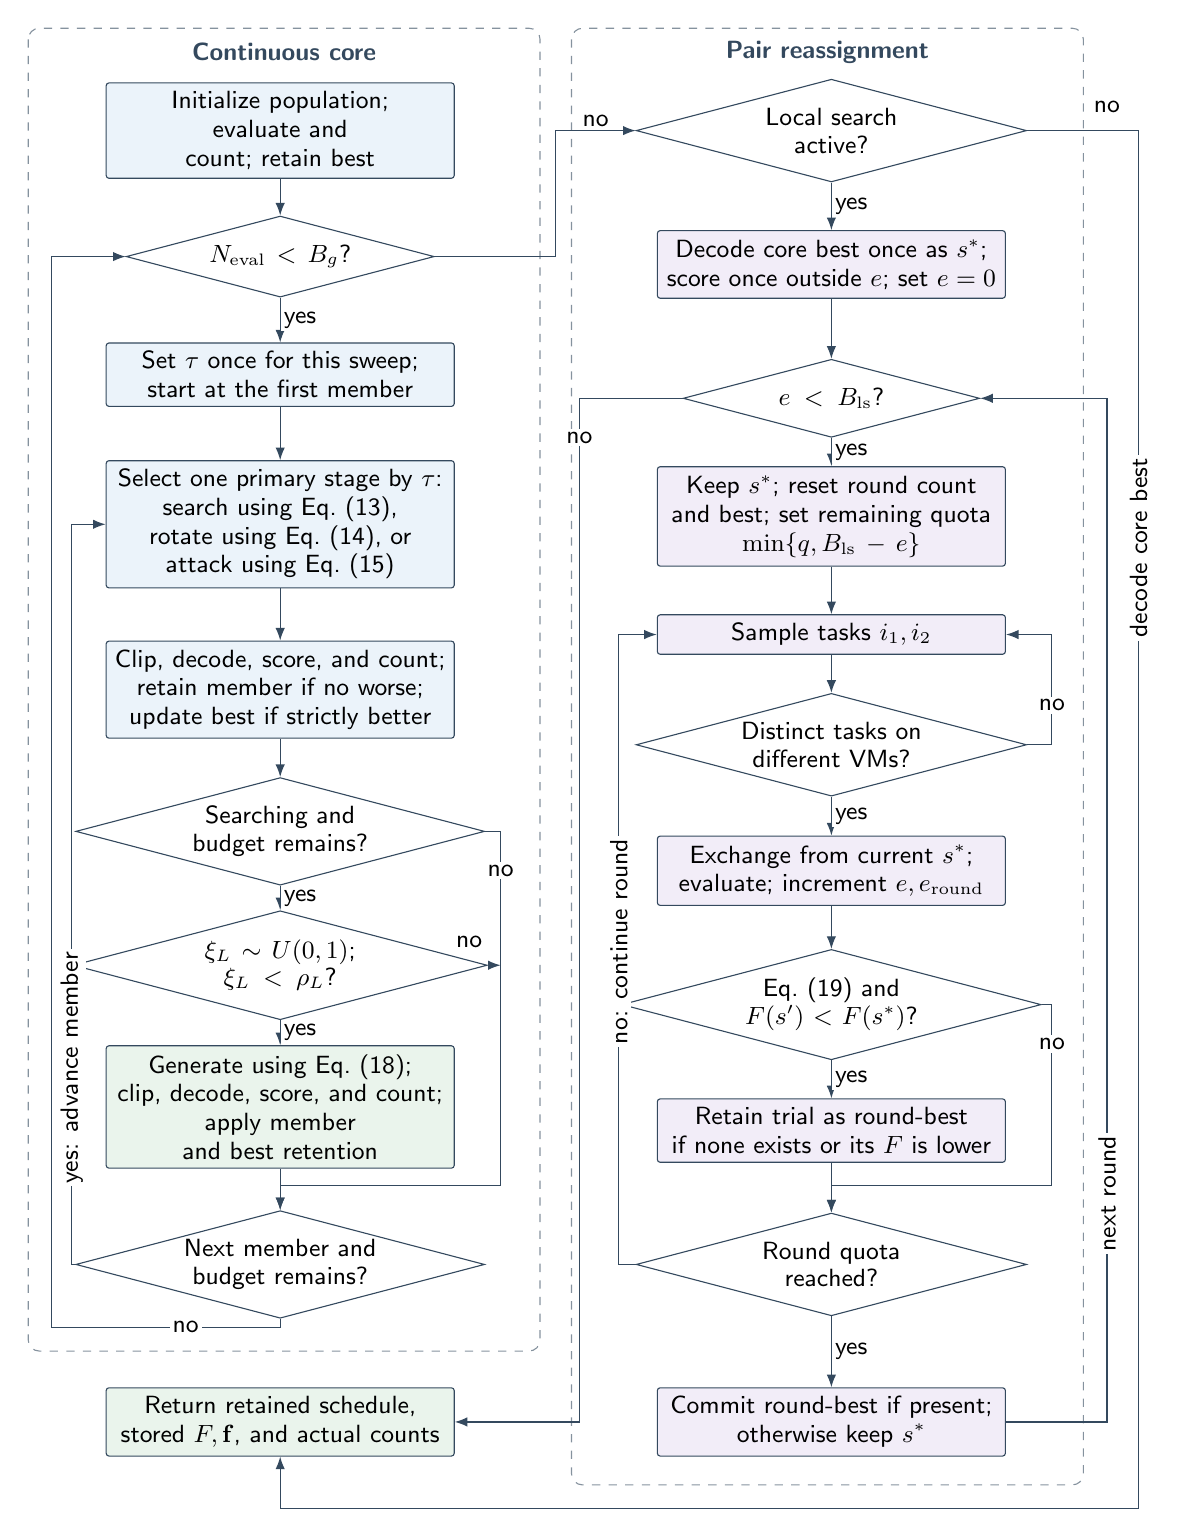
\begin{tikzpicture}[x=1mm,y=-1mm]
\draw[dashed,rounded corners,draw=ink!60] (0,-9) rectangle (65,159);
\draw[dashed,rounded corners,draw=ink!60] (69,-9) rectangle (134,176);
\node[title] at (32.5,-6) {Continuous core};
\node[title] at (101.5,-6) {Pair reassignment};

\node[box] (init) at (32,4) {Initialize population;\\evaluate and count; retain best};
\node[decision] (budget) at (32,20) {$N_{\mathrm{eval}}<B_g$?};
\node[box] (sweep) at (32,35) {Set $\tau$ once for this sweep;\\start at the first member};
\node[box] (stage) at (32,54) {Select one primary stage by $\tau$:\\search using Eq.~(\EqSearch),\\rotate using Eq.~(\EqRotation), or\\attack using Eq.~(\EqAttack)};
\node[box] (primary) at (32,75) {Clip, decode, score, and count;\\retain member if no worse;\\update best if strictly better};
\node[decision] (searching) at (32,93) {Searching and\\budget remains?};
\node[decision] (trigger) at (32,110) {$\xi_L\sim U(0,1)$;\\$\xi_L<\rho_L$?};
\node[box,fill=greenfill] (aux) at (32,128) {Generate using Eq.~(\EqLevy);\\clip, decode, score, and count;\\apply member and best retention};
\node[decision] (member) at (32,148) {Next member and\\budget remains?};
\draw[flow] (init) -- (budget);
\draw[flow] (budget) -- node[tag,right]{yes} (sweep);
\draw[flow] (sweep) -- (stage);
\draw[flow] (stage) -- (primary);
\draw[flow] (primary) -- (searching);
\draw[flow] (searching) -- node[tag,right]{yes} (trigger);
\draw[flow] (trigger) -- node[tag,right]{yes} (aux);
\draw[flow] (aux) -- (member);
\draw[flow] (searching.east) -- (60,93) -- (60,138) -- (32,138) -- (member.north);
\node[tag] at (60,98) {no};
\draw[flow] (trigger.east) -- (60,110);
\node[tag] at (56,107) {no};
\draw[flow] (member.west) -- (5.5,148) -- (5.5,54) -- (stage.west);
\node[tag,rotate=90] at (5.5,123) {yes: advance member};
\draw[flow] (member.south) -- (32,156) -- (3,156) -- (3,20) -- (budget.west);
\node[tag] at (20,156) {no};

\node[decision] (mode) at (102,4) {Local search\\active?};
\node[local] (handoff) at (102,21) {Decode core best once as $s^*$;\\score once outside $e$; set $e=0$};
\node[decision] (localbudget) at (102,38) {$e<B_{\mathrm{ls}}$?};
\node[local] (round) at (102,53) {Keep $s^*$; reset round count\\and best; set remaining quota\\$\min\{q,B_{\mathrm{ls}}-e\}$};
\node[local] (draw) at (102,68) {Sample tasks $i_1,i_2$};
\node[decision] (legal) at (102,82) {Distinct tasks on\\different VMs?};
\node[local] (trial) at (102,98) {Exchange from current $s^*$;\\evaluate; increment $e,e_{\mathrm{round}}$};
\node[decision] (safe) at (102,115) {Eq.~(\EqAccept) and\\$F(s')<F(s^*)$?};
\node[local] (best) at (102,131) {Retain trial as round-best\\if none exists or its $F$ is lower};
\node[decision] (quota) at (102,148) {Round quota\\reached?};
\node[local] (commit) at (102,168) {Commit round-best if present;\\otherwise keep $s^*$};
\node[box,fill=greenfill] (out) at (32,168) {Return retained schedule,\\stored $F,\mathbf{f}$, and actual counts};
\draw[flow] (budget.east) -- (67,20) -- (67,4) -- node[tag,above]{no} (mode.west);
\draw[flow] (mode) -- node[tag,right]{yes} (handoff);
\draw[flow] (handoff) -- (localbudget);
\draw[flow] (localbudget) -- node[tag,right]{yes} (round);
\draw[flow] (round) -- (draw);
\draw[flow] (draw) -- (legal);
\draw[flow] (legal) -- node[tag,right]{yes} (trial);
\draw[flow] (legal.east) -- (130,82) -- (130,68) -- (draw.east);
\node[tag] at (130,77) {no};
\draw[flow] (trial) -- (safe);
\draw[flow] (safe) -- node[tag,right]{yes} (best);
\draw[flow] (best) -- (quota);
\draw[flow] (safe.east) -- (130,115) -- (130,138) -- (102,138) -- (quota.north);
\node[tag] at (130,120) {no};
\draw[flow] (quota) -- node[tag,right]{yes} (commit);
\draw[flow] (quota.west) -- (75,148) -- (75,68) -- (draw.west);
\node[tag,rotate=90] at (75,107) {no: continue round};
\draw[flow] (commit.east) -- (137,168) -- (137,38) -- (localbudget.east);
\node[tag,rotate=90] at (137,139) {next round};
\draw[flow] (localbudget.west) -- (70,38) -- (70,168) -- (out.east);
\node[tag] at (70,43) {no};
\draw[flow] (mode.east) -- (141,4) -- (141,179) -- (32,179) -- (out.south);
\node[tag] at (137,1) {no};
\node[tag,rotate=90] at (141,57) {decode core best};
\end{tikzpicture}
\end{document}
